\documentclass{standalone}
\usepackage{tikz}

\usetikzlibrary{math,calc}


\begin{document}

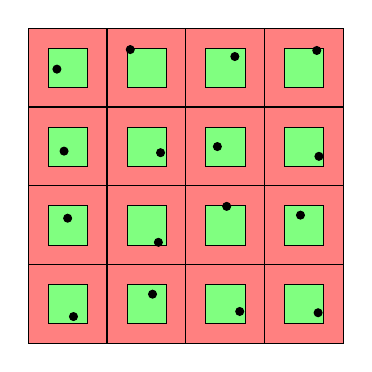
\begin{tikzpicture}
  \draw[fill=red!50] (0,0) rectangle (4,4);
  \draw (0,0) grid (4,4);

  \foreach \i in {1,2,3,4} {
    \foreach \j in {1,2,3,4} {
      \tikzmath{
        real \x;
        real \y;
        \x = \i - 0.25 - 0.5 * random();
        \y = \j - 0.25 - 0.5 * random();
      }

      \draw[ultra thin,fill=green!50] ($ (\i, \j) + (-0.25, -0.25) $) rectangle ++(-0.5, -0.5);

      \draw[fill=black] (\x, \y) circle [radius=0.05cm];
    }
  }
\end{tikzpicture}

\end{document}